\section{Networking}
The engine will support multiplayer.
As the customer wants the engine to follow the Unity engine API, the multiplayer system wil follow the multiplayer package of unity \textbf{Netcode}.

\subsection{Network library}
Multiple libraries have been considered, for example ENet, RakNet or Boost.
The uses library is SLikeNet. This library is a continuation of RakNet, which is a well known and well documented library.
The library is also easy to use and has a lot of features that are useful for the engine.

\subsection{Class diagram}
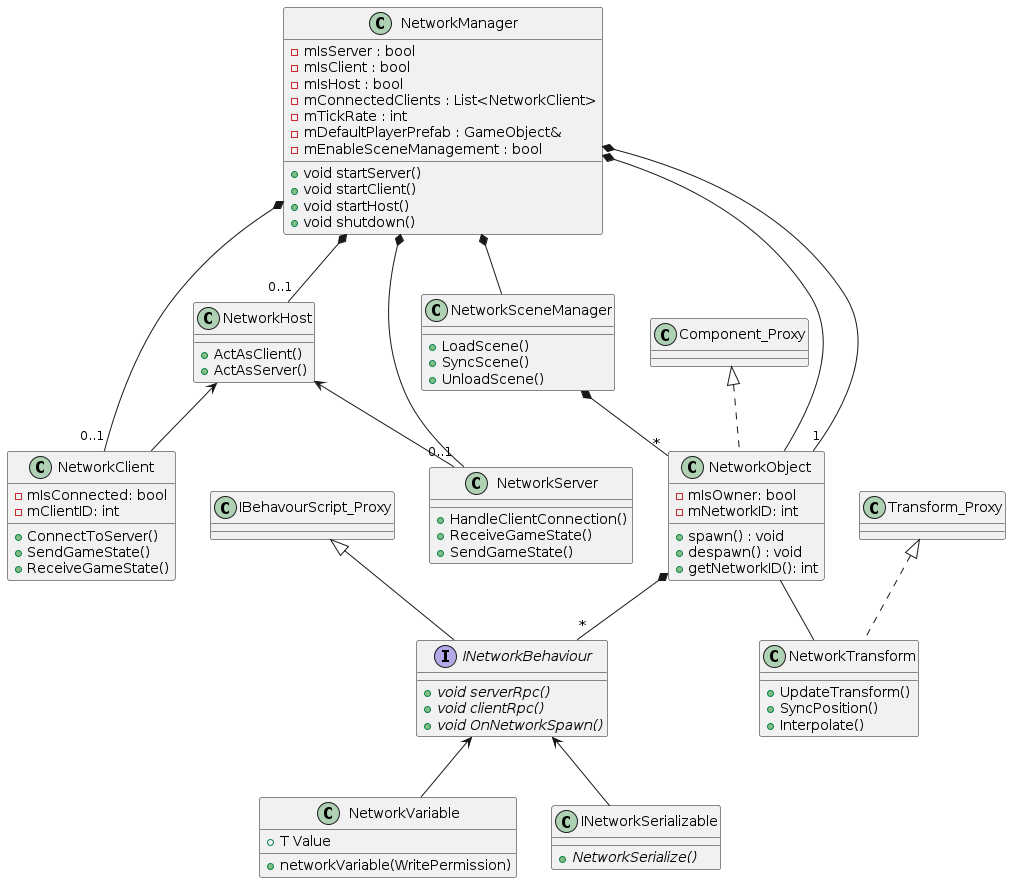
\includegraphics[width=\textwidth]{networkingClassDiagram.png}